% Prova dell'08/09/2022, esercizio 1: urto di un cuneo che incide sulla linea di scorrimento fra due correnti
% supersoniche alla stessa pressione. Numeri e figure: calcoli.py (stessa cartella).

\documentclass[11pt,a4paper]{article}

\usepackage[T1]{fontenc}
\usepackage[utf8]{inputenc}
\usepackage[italian]{babel}
\usepackage{amsmath,amssymb}
\usepackage[a4paper,margin=2.4cm]{geometry}
\usepackage{array}
\usepackage{siunitx}
\usepackage{booktabs}
\usepackage{graphicx}
\usepackage{float}
\usepackage{hyperref}

\hypersetup{hidelinks}
\setlength{\parindent}{0pt}
\setlength{\parskip}{4pt}
\allowdisplaybreaks
\graphicspath{{figure/}}
\sisetup{output-decimal-marker={,}, group-separator={\,}, per-mode=symbol,
         exponent-product=\cdot, range-phrase={\text{--}}}

\newcommand{\Cp}{C^{+}}
\newcommand{\Cm}{C^{-}}

\title{Gasdinamica -- Prova dell'08/09/2022, esercizio 1\\[2pt]
\large Urto di un cuneo che incide su una linea di scorrimento}
\author{}
\date{}

\begin{document}
\maketitle

\section*{Traccia}
Due flussi piani supersonici uniformi con pari pressioni e differenti numeri di Mach scorrono adiacenti.
Determinare l'effetto sul campo di moto del cuneo presente nella regione inferiore. Riportare quantitativamente il
fenomeno sui piani pressione--deviazione e odografo (valutazione 21/30).

Figura della traccia: corrente superiore $M_{\infty1}=3$, corrente inferiore $M_{\infty2}=8$ con $p_2=1$,
$\rho_2=1$, separate da una linea orizzontale; nella regione inferiore un cuneo con faccia superiore inclinata di
$\theta=\ang{20}$.

\begin{figure}[H]
  \centering
  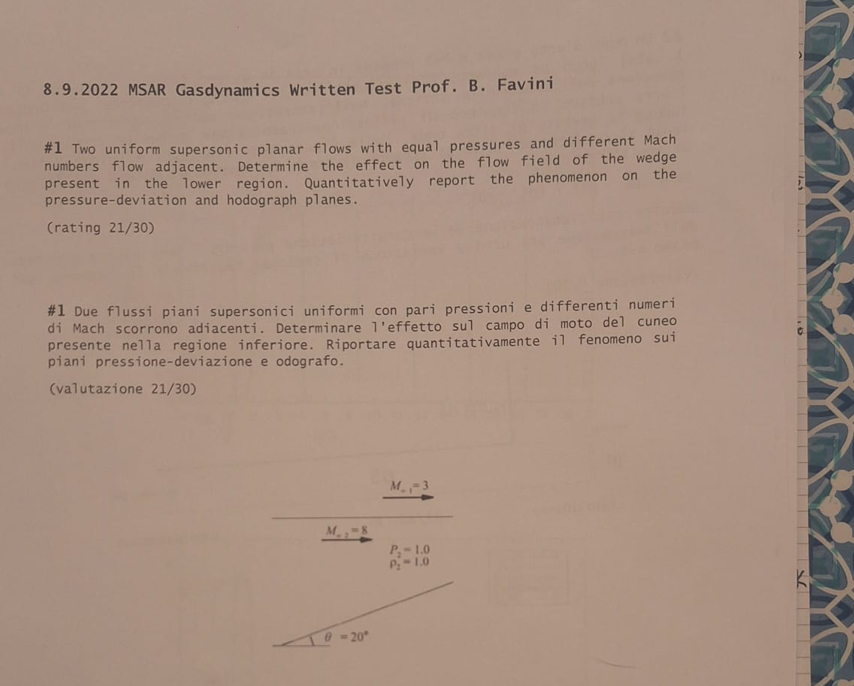
\includegraphics[width=0.55\textwidth]{originale.png}
  \caption{Traccia originale.}
\end{figure}

%==============================================================================
\section{Lettura del testo e dati}
Le due correnti sono separate da una \textbf{linea di scorrimento} orizzontale: stessa pressione e stessa direzione
($\theta=0$), ma Mach, velocità, densità ed entropia diverse. Il cuneo sta nella corrente inferiore, con la faccia
inferiore parallela alla corrente (non la disturba) e la faccia superiore che devia la corrente di \ang{20} verso
l'alto, verso la linea di scorrimento. Il cuneo è il solo elemento che rompe l'uniformità: si chiede come il suo
disturbo si propaga nelle due correnti.

Interpretazioni:
\begin{itemize}
\item gas: aria in entrambe le correnti, $\gamma=1{,}4$ (non indicato);
\item $p_1=p_2=1$ (``pari pressioni''); la densità della corrente superiore non è data, ma non serve: il piano
  $p$--$\theta$ dipende solo da $M$, $p$, $\theta$, e l'odografo si costruisce con le velocità adimensionali
  $u^*=u/a^*$, $v^*=v/a^*$, ciascuna corrente con il proprio $a^*$;
\item la quota $h$ della linea di scorrimento sul vertice O del cuneo non è data: le lunghezze sono riferite a $h$;
  la faccia del cuneo è abbastanza lunga da ricevere le onde riflesse.
\end{itemize}

\begin{table}[H]
  \centering
  \begin{tabular}{lll}
    \toprule
    Grandezza & Valore & Note \\
    \midrule
    $\gamma$ & \num{1.4} & aria, entrambe le correnti \\
    $M_1$, $p_1$, $\theta_1$ & $3$, $1$, \ang{0} & corrente superiore \\
    $M_2$, $p_2$, $\rho_2$, $\theta_2$ & $8$, $1$, $1$, \ang{0} & corrente inferiore ($a_2=\sqrt{\gamma p_2/\rho_2}=1{,}18$) \\
    $\theta_w$ & \ang{20} & faccia superiore del cuneo \\
    \bottomrule
  \end{tabular}
  \caption{Dati del problema (grandezze adimensionali).}
\end{table}

Tracce affini nel catalogo: B74-E01 (intersezione delle polari di due correnti supersoniche) e B51-E01 (incontro di
due correnti supersoniche, piani $p$--$\theta$ e odografo).

%==============================================================================
\section{Modello e ipotesi}
\begin{enumerate}
\item \textbf{Flusso piano, stazionario, non viscoso, gas perfetto.} La linea di scorrimento è una discontinuità
  di contatto: attraverso di essa $p$ e $\theta$ sono continue, mentre $M$, $V$, $\rho$ ed $s$ possono saltare.
  Trascuro lo strato di mescolamento che in realtà vi si sviluppa e lo strato limite sul cuneo.
\item \textbf{Tutte le regioni supersoniche} (da verificare, §8). Il problema è allora iperbolico: l'informazione
  viaggia solo lungo le caratteristiche, verso valle. Le onde sono urti obliqui, ventagli di Prandtl--Meyer e onde
  semplici, rappresentabili sul piano $p$--$\theta$ e sull'odografo.
\item \textbf{Urti sul ramo debole.} Il flusso è esterno e nessuna contropressione impone il ramo forte.
\item \textbf{Regioni omoentropiche.} Ogni urto incontrato finché è rettilineo dà alla corrente a valle entropia
  uniforme: nelle zone a valle valgono gli invarianti $\theta\pm\nu$ lungo le caratteristiche, e le onde semplici
  che vi si propagano sono esattamente isentropiche.
\item \textbf{Onde semplici rettilinee.} Per la geometria approssimo le caratteristiche di testa e di coda dei
  ventagli con semirette inclinate come negli stati uniformi adiacenti; le zone d'interazione fra ventagli di
  famiglie diverse non le risolvo punto per punto.
\end{enumerate}

%==============================================================================
\section{Analisi qualitativa}
\textbf{Urto del cuneo.} La faccia del cuneo devia la corrente 2 di \ang{20} verso l'alto. Poiché
$\theta_{\max}(M=8)=\ang{43.8}>\ang{20}$, nasce in O un \textbf{urto obliquo attaccato} della famiglia $\Cp$ (parete
sotto la corrente), sul ramo debole. L'urto sale e raggiunge la linea di scorrimento nel punto P.

\textbf{Interazione in P.} In P si incontrano la corrente 3 (dietro l'urto, $p_3\gg1$, $\theta=\ang{20}$) e la
corrente 1 ($p=1$, $\theta=0$): è un problema di Riemann stazionario. Le due correnti devono uscirne con la stessa
pressione e la stessa direzione. Nella corrente superiore, a bassa pressione, entra un'onda $\Cp$ di compressione:
l'\textbf{urto trasmesso}. Verso il basso torna un'onda $\Cm$, l'\textbf{onda riflessa}, la cui natura si stabilisce
così: se la linea di scorrimento restasse parallela al cuneo ($\theta=\ang{20}$), la polare di 1 darebbe
$p\approx3{,}8$, molto meno di $p_3\approx14{,}8$ (§7b). La corrente 3 deve quindi abbassare la propria pressione, e
lo può fare solo aumentando $\theta$: l'onda riflessa è un'\textbf{espansione centrata in P} e la linea di
scorrimento si inclina \textbf{più del cuneo}.

La corrente superiore si comporta come un contorno ``cedevole'', intermedio fra due casi limite: una parete rigida
orizzontale rifletterebbe un urto, un contorno a pressione costante ($p=1$, come il bordo di un getto) rifletterebbe
un'espansione fino a $p=1$. Una corrente a $M=3$ e $p=1$ cede molto a confronto della corrente 3, e il riflesso ha
la natura del secondo caso.

\textbf{Riflessioni successive.} Il ventaglio riflesso raggiunge la faccia del cuneo e si riflette con la stessa
natura (parete): una nuova espansione, $\Cp$, che riporta la corrente a \ang{20}. Questa raggiunge la linea di
scorrimento: si trasmette in alto come espansione e si riflette in basso come compressione (natura opposta, come
in P). La compressione torna sul cuneo, si riflette come compressione, e così via. A ogni interazione la linea di
scorrimento devia alternativamente sopra e sotto \ang{20}, con ampiezza decrescente. Lontano a valle la corrente
inferiore scorre in un canale delimitato dal cuneo e dalla linea di scorrimento, che si allineano: stato asintotico
a $\theta=\ang{20}$.

\textbf{Urto trasmesso.} La corrente superiore è illimitata: l'urto trasmesso non si riflette su nulla. È però
raggiunto, nel punto T, dal ventaglio d'espansione trasmesso alla seconda interazione, che lo indebolisce e lo
incurva.

%==============================================================================
\section{Topologia del campo}
\begin{figure}[H]
  \centering
  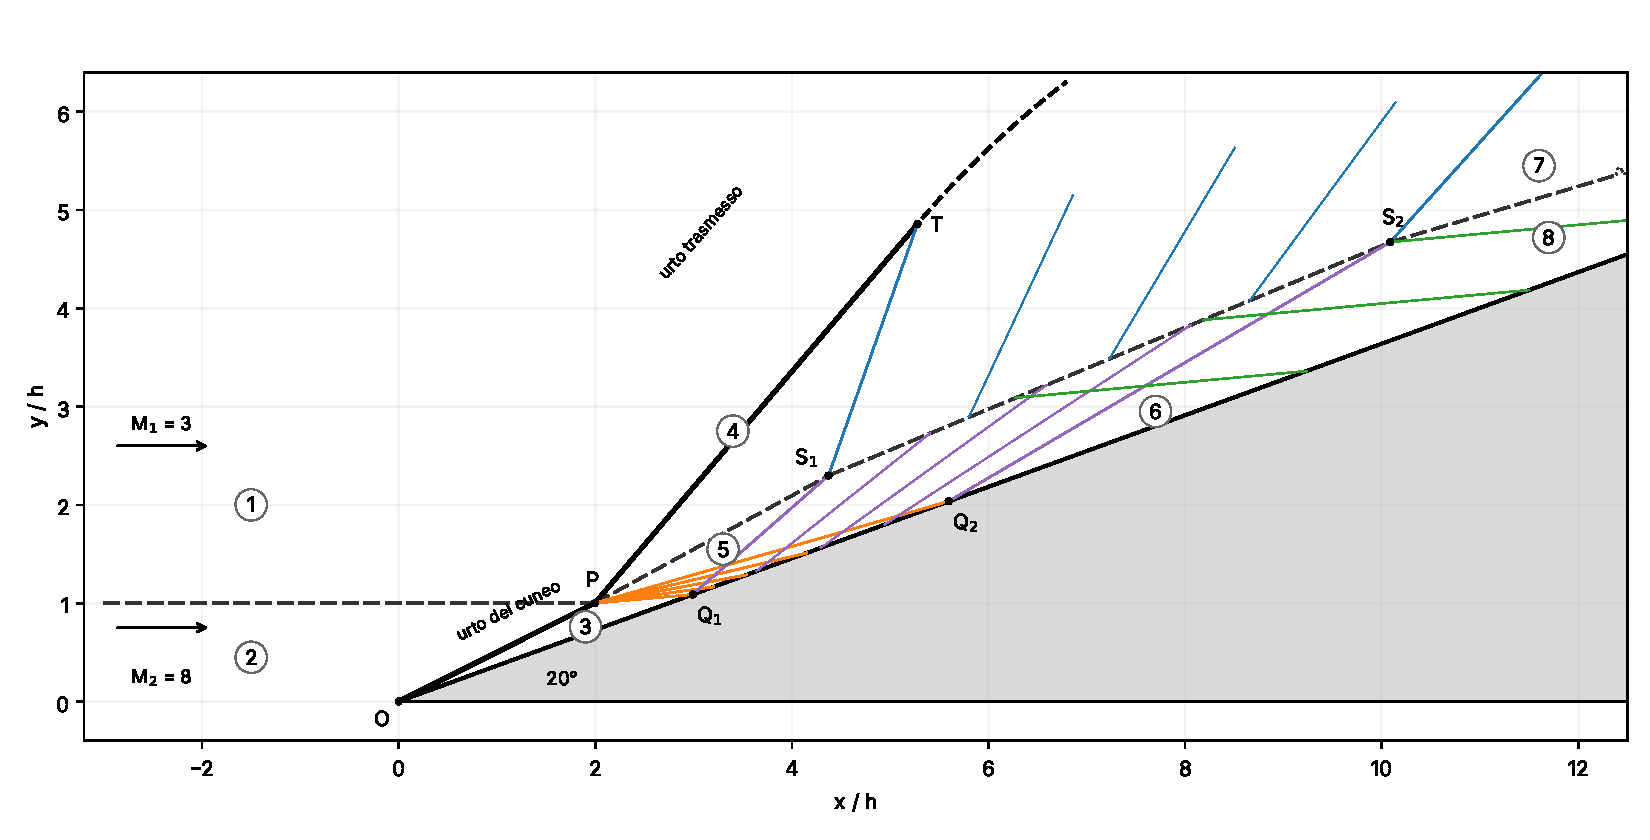
\includegraphics[width=\textwidth]{campo.pdf}
  \caption{Piano fisico, lunghezze riferite alla quota $h$ della linea di scorrimento (tratteggiata) sul vertice O.
  Nero: urti; arancio: ventaglio riflesso in P ($\Cm$); viola: ventaglio riflesso dal cuneo ($\Cp$); azzurro:
  ventaglio trasmesso nella corrente superiore; verde: compressioni riflesse alla seconda interazione. Oltre
  S$_2$ la linea di scorrimento oscilla, smorzandosi, attorno a \ang{20} (puntinata, qualitativa).}
  \label{fig:campo}
\end{figure}

\begin{table}[H]
  \centering
  \small
  \begin{tabular}{clll}
    \toprule
    Stato & Regione & Onda che lo genera & Natura \\
    \midrule
    1 & sopra, indisturbata & -- & -- \\
    2 & sotto, indisturbata & -- & -- \\
    3 & fra urto del cuneo e cuneo & urto in O, $\Cp$ & compressione (urto) \\
    4 & sopra, dietro l'urto trasmesso & urto in P, $\Cp$ & compressione (urto) \\
    5 & sotto, fra ventaglio in P e linea di scorr. & ventaglio in P, $\Cm$ & espansione \\
    6 & sotto, dopo la riflessione sul cuneo & ventaglio dal cuneo, $\Cp$ & espansione \\
    7 & sopra, dopo il ventaglio trasmesso (S$_1$--S$_2$) & ventaglio trasmesso, $\Cp$ & espansione \\
    8 & sotto, dopo la compressione riflessa & compressione, $\Cm$ & urto debole \\
    9 & sotto, a parete, dopo la sua riflessione & compressione, $\Cp$ & urto debole \\
    $\infty$ & stato asintotico, sopra e sotto & -- & -- \\
    \bottomrule
  \end{tabular}
  \caption{Stati e onde. Sulla linea di scorrimento: $p_4=p_5$, $\theta_4=\theta_5$; $p_7=p_8$, $\theta_7=\theta_8$.}
\end{table}

%==============================================================================
\section{Bilancio equazioni/incognite}
In P le incognite sono gli stati 4 e 5. Ciascuna onda lega pressione e deviazione dello stato a valle a quelle dello
stato a monte (polare d'urto per l'urto trasmesso, invariante $\theta-\nu$ e isentropica per il ventaglio): due
relazioni $p_4(\theta_4)$ e $p_5(\theta_5)$. La linea di scorrimento aggiunge $p_4=p_5$ e $\theta_4=\theta_5$. Quattro
equazioni in quattro incognite ($p_4,\theta_4,p_5,\theta_5$), cioè l'intersezione di due curve sul piano
$p$--$\theta$: un'equazione non lineare in una incognita, che risolvo per tentativi. Lo stesso vale per la seconda
interazione (stati 7 e 8). Sul cuneo, invece, la condizione $\theta=\ang{20}$ e l'invariante bastano: gli stati 6 e 9
si trovano direttamente.

%==============================================================================
\section{Scorciatoie fisiche}
\begin{itemize}
\item Le regioni sono supersoniche, quindi la corrente superiore non può influenzare ciò che sta a monte delle
  caratteristiche uscenti da P: urto del cuneo e stato 3 si calcolano come se il cuneo fosse isolato.
\item Lo stato asintotico non richiede di seguire tutte le riflessioni: la linea di scorrimento finisce parallela
  al cuneo, quindi la corrente superiore, a valle dell'urto trasmesso, ha ruotato complessivamente da $\theta_4$ a
  \ang{20} attraverso onde deboli. Approssimandole come isentropiche, $p_\infty$ segue dall'invariante (§7e).
\end{itemize}

%==============================================================================
\section{Calcolo}

\subsection*{a) Urto del cuneo: stato 3}
Dalla relazione $\theta$--$\sigma$--$M$ con $M_2=8$ e $\theta=\ang{20}$ (ramo debole):
\[
\tan\theta=2\cot\sigma\,\frac{M_2^2\sin^2\sigma-1}{M_2^2(\gamma+\cos2\sigma)+2}
\ \Rightarrow\ \sigma_3=\ang{26.6},\qquad M_{n2}=8\sin\ang{26.6}=3{,}58 .
\]
\[
\frac{p_3}{p_2}=1+\frac{2\gamma}{\gamma+1}(M_{n2}^2-1)=1+1{,}167\,(12{,}85-1)=14{,}8,\qquad
\frac{\rho_3}{\rho_2}=\frac{2{,}4\cdot12{,}85}{0{,}4\cdot12{,}85+2}=4{,}32,
\]
\[
M_{n3}^2=\frac{1+\delta M_{n2}^2}{\gamma M_{n2}^2-\delta}=\frac{1+0{,}2\cdot12{,}85}{1{,}4\cdot12{,}85-0{,}2}=0{,}201,
\qquad M_3=\frac{M_{n3}}{\sin(\sigma_3-\theta)}=\frac{0{,}448}{\sin\ang{6.62}}=3{,}89 .
\]
Stato 3: $p_3=14{,}8$, $\rho_3=4{,}32$, $M_3=3{,}89$, $\theta_3=\ang{20}$, $\nu_3=\nu(3{,}89)=\ang{64.3}$,
$\mu_3=\arcsin(1/M_3)=\ang{14.9}$. Pressione totale:
$p_{03}=p_3(1+\delta M_3^2)^{3{,}5}=14{,}8\cdot4{,}02^{3{,}5}=1933$.

L'urto incontra la linea di scorrimento a $x_P=h/\tan\sigma_3=2{,}0\,h$.

\subsection*{b) Prima interazione in P: stati 4 e 5}
Prendo come incognita l'angolo $\sigma$ dell'urto trasmesso, che parametrizza la polare di 1. Per ogni tentativo:
\begin{enumerate}
\item urto trasmesso: $M_n=3\sin\sigma$, $p_4=1+1{,}167\,(M_n^2-1)$, $\theta_4$ dalla relazione
  $\theta$--$\sigma$--$M$ con $M_1=3$;
\item ventaglio riflesso ($\Cm$, isentropico, $\theta-\nu$ costante): $p_5=p_4$, quindi
  $1+\delta M_5^2=(p_{03}/p_4)^{1/3{,}5}$, poi $\theta_5=\theta_3+\nu(M_5)-\nu_3$;
\item controllo: $\theta_4-\theta_5$.
\end{enumerate}
Primo tentativo: linea di scorrimento parallela al cuneo, $\theta_4=\ang{20}$, cioè $\sigma=\ang{37.8}$. Il secondo
tentativo, $\sigma=\ang{50}$, tiene conto che il primo dà $\theta_5\gg\theta_4$; poi interpolazione lineare fra gli
ultimi due:
\begin{table}[H]
  \centering
  \small
  \begin{tabular}{cccccccc}
    \toprule
    $\sigma$ & $M_n$ & $p_4=p_5$ & $\theta_4$ & $M_5$ & $\nu_5$ & $\theta_5$ & $\theta_4-\theta_5$ \\
    \midrule
    \ang{37.76} & 1,837 & 3,771 & \ang{20.00} & 4,973 & \ang{76.66} & \ang{32.41} & \ang{-12.41} \\
    \ang{50.00} & 2,298 & 5,995 & \ang{28.86} & 4,587 & \ang{72.78} & \ang{28.52} & \ang{+0.34} \\
    \ang{49.68} & 2,287 & 5,937 & \ang{28.67} & 4,595 & \ang{72.87} & \ang{28.61} & \ang{+0.06} \\
    \ang{49.61} & 2,285 & 5,924 & \ang{28.63} & 4,597 & \ang{72.88} & \ang{28.63} & \ang{0.00} \\
    \bottomrule
  \end{tabular}
  \caption{Tentativi sull'angolo dell'urto trasmesso.}
\end{table}
Il primo tentativo conferma l'analisi qualitativa: con $\theta=\ang{20}$ la corrente superiore regge solo $p=3{,}77$,
e la corrente 3 per scendere a quella pressione dovrebbe ruotare fino a \ang{32}. All'ultimo tentativo la differenza
è sotto \ang{0.01}: la soluzione è raggiunta.

\textbf{Stato 4} (urto trasmesso, $\sigma=\ang{49.6}$, $M_n=2{,}28$):
\[
p_4=5{,}92,\qquad \theta_4=\ang{28.6},
\]
\[
M_{n4}^2=\frac{1+0{,}2\cdot5{,}22}{1{,}4\cdot5{,}22-0{,}2}=0{,}288,\qquad
M_4=\frac{0{,}536}{\sin(\ang{49.6}-\ang{28.6})}=1{,}50,
\]
con $p_{04}/p_{01}=0{,}590$, quindi $p_{04}=0{,}590\cdot1\cdot(1+0{,}2\cdot9)^{3{,}5}=21{,}7$.

\textbf{Stato 5} (ventaglio $\Cm$ centrato in P): $p_5=5{,}92$, $M_5=4{,}60$, $\theta_5=\theta_3+\nu_5-\nu_3=
\ang{20}+\ang{72.9}-\ang{64.3}=\ang{28.6}$, $\mu_5=\ang{12.6}$. Il ventaglio va dalla testa inclinata di
$\theta_3-\mu_3=\ang{5.1}$ alla coda inclinata di $\theta_5-\mu_5=\ang{16.1}$: entrambe meno inclinate del cuneo, quindi
lo raggiungono, in Q$_1$ ($x\approx3{,}0\,h$) e Q$_2$ ($x\approx5{,}6\,h$).

La linea di scorrimento si inclina di $\theta_4=\ang{28.6}$, \ang{8.6} più del cuneo.

\subsection*{c) Riflessione del ventaglio sul cuneo: stato 6}
La parete impone $\theta_6=\ang{20}$. L'onda riflessa è $\Cp$, quindi attraverso di essa $\theta+\nu$ è costante:
\[
\nu_6=\nu_5+(\theta_5-\theta_6)=\ang{72.9}+\ang{8.6}=\ang{81.5}\ \Rightarrow\ M_6=5{,}53,
\]
\[
p_6=\frac{p_{03}}{(1+\delta M_6^2)^{3{,}5}}=\frac{1933}{(1+0{,}2\cdot5{,}53^2)^{3{,}5}}=\frac{1933}{965}=2{,}00 .
\]
È di nuovo un'espansione: lo stato 6 è a pressione molto più bassa del 3. Testa e coda del ventaglio riflesso,
nelle regioni 5 e 6: $\theta_5+\mu_5=\ang{41.2}$ e $\theta_6+\mu_6=\ang{30.4}$. La testa raggiunge la linea di
scorrimento in S$_1$ ($x\approx4{,}4\,h$), prima che il ventaglio incidente abbia finito di riflettersi: fra Q$_1$,
Q$_2$ e la linea di scorrimento i due ventagli interagiscono, e lì la soluzione non è analitica. Basta osservare che
lungo il cuneo, fra Q$_1$ e Q$_2$, la pressione scende con continuità da $p_3$ a $p_6$.

\subsection*{d) Seconda interazione: stati 7 e 8}
Ora la corrente superiore (stato 4, $p_4=5{,}92$) è a pressione più alta di quella inferiore (stato 6, $p_6=2{,}00$):
in alto passa un'espansione $\Cp$, in basso torna una compressione $\Cm$. Con lo stesso procedimento di §7b,
partendo da $\theta_4$ e $\theta_6$:
\[
\text{sopra: } \nu_7=\nu_4+(\theta_4-\theta_7),\qquad
\text{sotto: urto debole da 6 con deviazione } \theta_6-\theta_8,\qquad p_7=p_8,\ \theta_7=\theta_8,
\]
si trova
\[
p_7=p_8=3{,}17,\qquad \theta_7=\theta_8=\ang{16.5},\qquad M_7=1{,}91,\quad M_8=5{,}11 .
\]
La compressione riflessa è debolissima ($M_n=1{,}22$): trattata come isentropica darebbe $\theta=\ang{16.53}$ invece di
\ang{16.52}. Riflessa a sua volta dal cuneo ($\theta_9=\ang{20}$), porta la pressione a parete a $p_9=4{,}86$
($M_9=4{,}74$).

La linea di scorrimento devia dunque da \ang{28.6} a \ang{16.5}: lo scarto da \ang{20} passa da $+\ang{8.6}$ a
$-\ang{3.5}$. Il rapporto $-3{,}5/8{,}6\approx-0{,}4$ misura lo smorzamento a ogni ciclo di riflessioni. Lo stesso valore si
ottiene dalle pendenze delle curve $p$--$\theta$ ai due lati della linea di scorrimento,
$K=\gamma pM^2/\sqrt{M^2-1}$: $K_4=16{,}7$ e $K_5=39{,}1$ danno $(K_5-K_4)/(K_5+K_4)=0{,}40$.

\subsection*{e) Stato asintotico}
Lontano a valle la linea di scorrimento e la corrente inferiore sono parallele al cuneo: $\theta_\infty=\ang{20}$.
La corrente superiore, dopo l'urto trasmesso, ha attraversato solo onde deboli $\Cp$ (con $\theta+\nu$ costante),
dunque
\[
\nu_\infty=\nu_4+(\theta_4-\ang{20})=\ang{11.8}+\ang{8.6}=\ang{20.5}\ \Rightarrow\ M_{\infty,\rm sopra}=1{,}79,
\]
\[
p_\infty=\frac{p_{04}}{(1+\delta M_\infty^2)^{3{,}5}}=\frac{21{,}7}{(1+0{,}2\cdot1{,}79^2)^{3{,}5}}\approx3{,}82 .
\]
La corrente inferiore, a $p_\infty$ e con la pressione totale dello stato 3:
$(1+\delta M^2)^{3{,}5}=p_{03}/p_\infty=505$, quindi $M_{\infty,\rm sotto}\approx4{,}96$. Le pressioni a parete
oscillano attorno a questo valore: $p_6=2{,}00<p_\infty<p_9=4{,}86$.

%==============================================================================
\section{Verifiche a posteriori}
\begin{itemize}
\item Urti attaccati: $\ang{20}<\theta_{\max}(8)=\ang{43.8}$ e $\ang{28.6}<\theta_{\max}(3)=\ang{34.1}$. \emph{Verificata.}
\item Urti di compressione con $M_n>1$ (entropia crescente): cuneo 3,58, trasmesso 2,28, compressioni riflesse
  1,22 e 1,21. \emph{Verificata.}
\item Natura dell'onda riflessa in P: $p_5=5{,}92<p_3=14{,}8$, espansione come previsto. \emph{Verificata.}
\item Regioni supersoniche (modello stazionario 2D lecito): il minimo è $M_4=1{,}50$. \emph{Verificata.}
\item Ramo debole: le polari di 1 e 3 si intersecano anche in $p=10{,}0$, $\theta=\ang{23.9}$, sul ramo forte della
  polare di 1 ($M_4<1$). Senza contropressione a valle la soluzione è quella debole. \emph{Scartata la forte.}
\item Raccordo sulla linea di scorrimento: $|\theta_4-\theta_5|<\ang{0.01}$, $p_4=p_5$. \emph{Verificata.}
\item Assenza del vuoto: $\nu_6=\ang{81.5}<\nu_{\max}=\ang{130.5}$. \emph{Verificata.}
\item Geometria: testa e coda del ventaglio in P (\ang{5.1}, \ang{16.1}) meno inclinate del cuneo, quindi lo
  raggiungono. \emph{Verificata.}
\item Stato asintotico isentropico nella corrente superiore: le onde dopo l'urto trasmesso hanno $M_n\le1{,}22$,
  salto d'entropia trascurabile. \emph{Coerente.}
\end{itemize}

%==============================================================================
\section{Risultati}
\begin{table}[H]
  \centering
  \small
  \begin{tabular}{cccccccl}
    \toprule
    Stato & $M$ & $p$ & $\theta$ & $\nu$ & $M^*$ & $p_0$ & \\
    \midrule
    1 & 3,00 & 1 & \ang{0} & \ang{49.8} & 1,96 & 36,7 & dato \\
    2 & 8,00 & 1 & \ang{0} & \ang{95.6} & 2,36 & 9763 & dato \\
    3 & 3,89 & 14,8 & \ang{20} & \ang{64.3} & 2,12 & 1933 & esatto \\
    4 & 1,50 & 5,92 & \ang{28.6} & \ang{11.8} & 1,36 & 21,7 & esatto \\
    5 & 4,60 & 5,92 & \ang{28.6} & \ang{72.9} & 2,20 & 1933 & esatto \\
    6 & 5,53 & 2,00 & \ang{20} & \ang{81.5} & 2,27 & 1933 & esatto \\
    7 & 1,91 & 3,17 & \ang{16.5} & \ang{23.9} & 1,59 & 21,7 & esatto \\
    8 & 5,11 & 3,17 & \ang{16.5} & \ang{78.0} & 2,24 & 1914 & esatto \\
    $\infty$ sopra & 1,79 & $\approx3{,}82$ & \ang{20} & \ang{20.5} & 1,53 & 21,7 & stima \\
    $\infty$ sotto & 4,96 & $\approx3{,}82$ & \ang{20} & \ang{76.5} & 2,23 & 1933 & stima \\
    \bottomrule
  \end{tabular}
  \caption{Stati del campo. ``Esatto'' nel modello non viscoso; lo stato asintotico usa l'approssimazione
  isentropica delle onde deboli. $M^*=V/a^*$ con l'$a^*$ della propria corrente.}
\end{table}
Onde: urto del cuneo $\sigma_3=\ang{26.6}$, $p_3/p_2=14{,}8$; urto trasmesso $\sigma=\ang{49.6}$, $p_4/p_1=5{,}92$;
espansione riflessa in P di \ang{8.6} ($p_5/p_3=0{,}40$); espansione riflessa dal cuneo di \ang{8.6}
($p_6/p_5=0{,}34$); linea di scorrimento inclinata di \ang{28.6}, poi \ang{16.5}, asintoticamente \ang{20}.

%==============================================================================
\section{Rappresentazioni}
\begin{figure}[H]
  \centering
  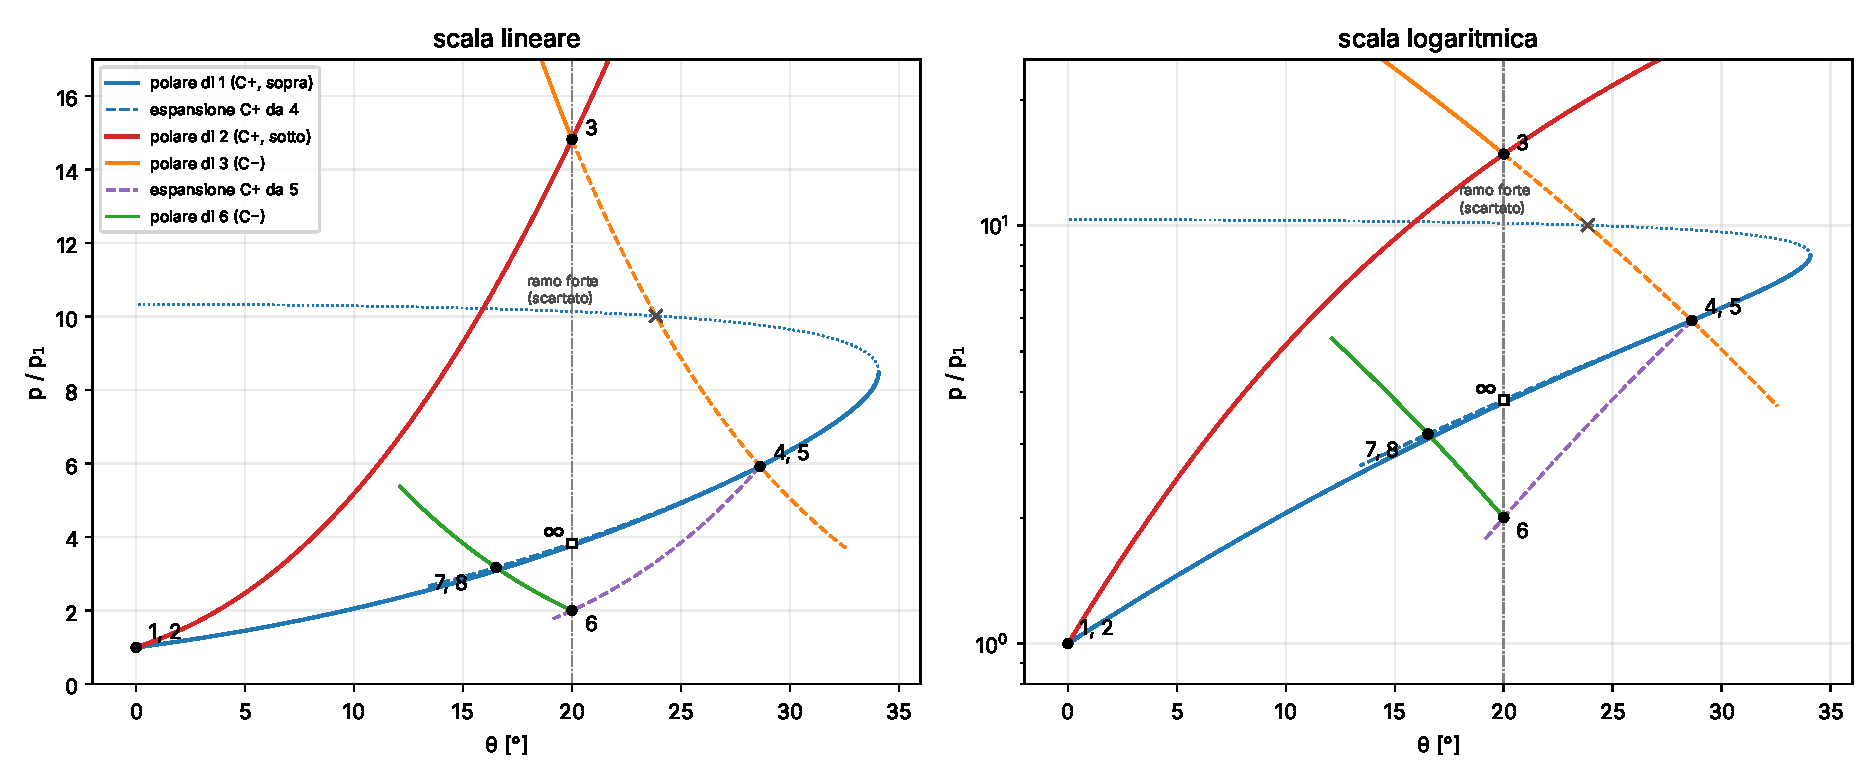
\includegraphics[width=\textwidth]{p_theta.pdf}
  \caption{Piano $p$--$\theta$ in scala lineare (sinistra) e logaritmica (destra). Ramo debole continuo, ramo forte
  puntinato, espansioni tratteggiate; la retta verticale è la parete del cuneo ($\theta=\ang{20}$).}
  \label{fig:pt}
\end{figure}
Lettura del piano $p$--$\theta$: la polare di 2 (rossa) sale ripidissima perché $M_2=8$, e sulla retta
$\theta=\ang{20}$ dà lo stato 3. Da 3 partono le due curve della famiglia $\Cm$: urto verso sinistra (pressioni
maggiori, $\theta$ minori) ed espansione verso destra. L'intersezione con la polare di 1 (azzurra) è 4--5: avviene sul
ramo d'espansione di 3, perché la polare di 1 è molto più bassa e piatta. È il motivo per cui l'onda riflessa è
un'espansione: la corrente superiore, a parità di deviazione, sviluppa molta meno pressione della 3. Da 5
l'espansione $\Cp$ torna sulla retta della parete in 6; da 6 la polare $\Cm$ (verde) incontra l'espansione $\Cp$ di 4
in 7--8. Gli stati successivi si avvolgono attorno al punto $\infty$, sulla retta \ang{20} e sull'espansione di 4.
L'intersezione sul ramo forte della polare di 1 è segnata e scartata.

Le pressioni vanno da 1 a 14,8. In scala lineare si vede bene la differenza di ``rigidezza'' delle due correnti (la
pendenza delle curve), ma gli stati 6--9 e $\infty$ si addensano in basso. La scala logaritmica separa questi stati e
mostra le oscillazioni attorno a $p_\infty$; deforma però la concavità del ramo debole delle polari.

\begin{figure}[H]
  \centering
  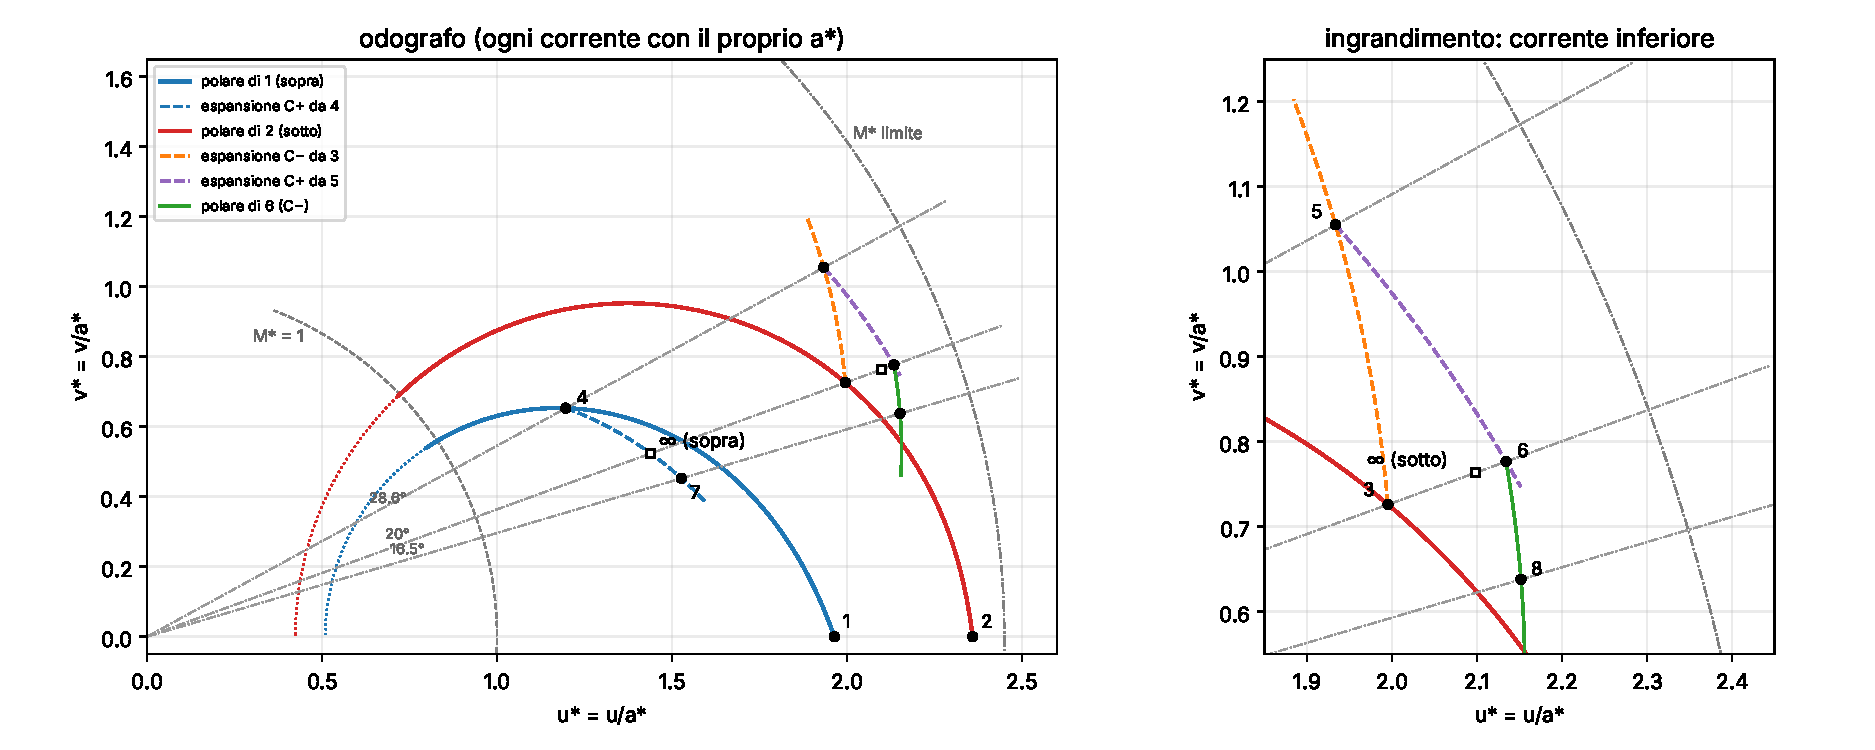
\includegraphics[width=\textwidth]{odografo.pdf}
  \caption{Odografo $(u^*,v^*)$, ogni corrente adimensionalizzata con il proprio $a^*$; cerchio sonico $M^*=1$ e
  cerchio limite $M^*=\sqrt{(\gamma+1)/(\gamma-1)}=2{,}45$. A destra l'ingrandimento della corrente inferiore. Le
  semirette dall'origine sono le direzioni \ang{20}, \ang{28.6} e \ang{16.5}.}
  \label{fig:odo}
\end{figure}
Sull'odografo gli urti stanno sulle strofoidi (polari d'urto) di 1 e 2, le espansioni sulle epicicloidi. Lo stato 2
è vicino al cerchio limite ($M^*=2{,}36$ su 2,45): la corrente inferiore ha già quasi tutta l'entalpia in forma
cinetica, e ogni onda la sposta poco in modulo. Nell'ingrandimento: 3 sulla polare di 2 lungo la semiretta \ang{20};
l'espansione $\Cm$ porta a 5 (modulo maggiore, direzione \ang{28.6}); l'espansione $\Cp$ riporta a 6 sulla semiretta
\ang{20}; l'urto debole da 6 scende a 8 sulla semiretta \ang{16.5}. Per la corrente superiore lo stato 4 sta sulla
polare di 1 lungo la stessa semiretta \ang{28.6} di 5: la condizione della linea di scorrimento si legge
sull'odografo come stessa direzione, con modulo diverso. Da 4 l'epicicloide porta a 7 (\ang{16.5}) e oltre fino a
$\infty$ (\ang{20}).

%==============================================================================
\section{Discussione fisica}
\textbf{Effetto del cuneo.} Il disturbo del cuneo non resta confinato nella corrente inferiore: attraverso la linea di
scorrimento produce un urto obliquo nella corrente superiore ($p\approx5{,}9$ volte quella indisturbata) e deflette
la linea di scorrimento oltre l'inclinazione del cuneo (\ang{28.6}). La corrente superiore è ``cedevole'' rispetto
alla 3. Per onde deboli, dalle relazioni di compatibilità, la pressione cresce con la deviazione come
$dp/d\theta=\gamma pM^2/\sqrt{M^2-1}$ ($\theta$ in radianti): 4,5 per la corrente 1 contro 83 per la 3. Per
questo l'urto del cuneo si riflette come espansione, come farebbe sul bordo di un getto, e non come urto, come
farebbe su una parete. Una parete orizzontale al posto della corrente 1 darebbe un urto riflesso con $p\approx75$; un
contorno a $p=1$ un'espansione fino a $\theta=\ang{42}$. La corrente a $M=3$ dà una soluzione intermedia, molto più
vicina al contorno libero.

\textbf{Pressione sul cuneo.} Il carico sul cuneo non è quello del cuneo isolato ($p_3=14{,}8$ ovunque): resta $p_3$
solo da O a Q$_1$, poi scende a $p_6=2{,}0$ (oltre Q$_2$), risale a $p_9=4{,}9$ e oscilla smorzandosi verso
$p_\infty\approx3{,}8$. L'espansione riflessa scarica quindi gran parte della faccia del cuneo.

\textbf{Campo lontano.} Lo stato asintotico è a $\theta=\ang{20}$ come se la corrente superiore fosse stata deviata di
\ang{20} da un urto unico, ma non coincide con quel caso: l'urto unico darebbe $p=3{,}77$, $M=1{,}99$ e
$p_0/p_{01}=0{,}80$; il percorso reale (urto a \ang{28.6} e poi espansioni) dà $p_\infty\approx3{,}82$,
$M_\infty=1{,}79$ e $p_0/p_{01}=0{,}59$. Lo ``scavalcamento'' iniziale della linea di scorrimento costa pressione
totale alla corrente superiore. L'urto trasmesso, raggiunto in T dal ventaglio trasmesso, si incurva e si indebolisce:
dietro il suo tratto curvo la corrente superiore non è più uniforme né omoentropica.

\textbf{Limiti del modello.} In realtà la linea di scorrimento è uno strato di mescolamento che si allarga verso
valle (il salto di velocità fra le due correnti è grande), e lo strato limite sul cuneo interagisce con le onde
riflesse: le riflessioni successive, sempre più deboli, si confondono rapidamente con questi effetti viscosi. Restano
significativi l'urto trasmesso, la prima deviazione della linea di scorrimento e la caduta di pressione sul cuneo.

\end{document}
